% Essential Formatting

\documentclass[12pt]{article}
\usepackage{epsfig,amsmath,amsthm,amssymb,textcomp}
\usepackage[questions, answersheet]{../../urmathtest}[2001/05/12]
%\usepackage[answersheet]{urmathtest}[2001/05/12]
%\usepackage[answers]{urmathtest}[2001/05/12]


% For use with pdflatex
% \pdfpagewidth\paperwidth
% \pdfpageheight\paperheight

% Basic User Defs

\def\ds{\displaystyle}

\newcommand{\ansbox}[1]
{\work{
  \pos\hfill \framebox[#1][l]{ANSWER:\rule[-.3in]{0in}{.7in}}
}{}}

\newcommand{\ansrectangle}
{\work{
  \pos\hfill \framebox[6in][l]{ANSWER:\rule[-.3in]{0in}{.7in}}
}{}}


% Beginning of the Document

\begin{document}
\examtitle{DATA MINING W4240}{HOMEWORK 2}{09/14/2010}

\begin{center}
	Professor: Frank Wood
\end{center}

% Problems Start Here % ----------------------------------------------------- %

{\bf Preliminary Instructions}

\begin{enumerate}
	\item Download the skeleton code for the assignment at \\  http://www.stat.columbia.edu/$\sim$fwood/w4240/Homework/index.html
	\item Unzip the downloaded material in an appropriate folder, something like w4240/hw2/
	\item Ignore files with extra extensions, not just .m.  These are somehow created with the tar and I don't know how to get rid of them.
	\item Open MATLAB and navigate to the folder containing the downloaded material
\end{enumerate}

For this homework the code is quite a bit more complex.  Graphical data structures that are useful for graphical models are difficult to deal with unless you use certain semi-advanced programing techniques such as recursion and an object oriented programming style. You will not have to program these things yourself, but you will be much more likely to complete the project correctly if you understand the concepts.  Recursion is simply when a function calls itself.  When writing general functions to operate on graphs the concept is useful if you want to do an operation, such as message passing, for every node in the graph.  \\

Object oriented programing is a paradigm where you write code to define generic objects and then ``instantiate" instances of those objects to perform a task.  Generic object definitions are called classes.  For instance, you might write code to define a variable node and then when creating a graphical model you could instantiate the appropriate number of them.  Objects usually have fields and methods associated with them.  Fields are properties, such as if a node has been observed or not or the messages a node has received.  Methods are functions associated with the object which can act on the properties of the object and can take outside arguments.  For example, you might wish to ask an instantiated node for a message.  You would probably pass in the node you want the message to.  The node will have as properties the most recent messages it has received and can then calculate the correct message to return. \\

I expect this HW to be quit a difficult task due to the programming component.  Your grades will take into account the difficulty of the task.  Work first on part I and then concentrate on part II.

\problem{65}{

	The first part of the homework consists of implementing key parts of the sum-product algorithm for inference in discrete graphical models.  Only one type of object is used in this code base, namely the {\bf node} object.  The node class file does not need to be edited, but you should look at it to understand its properties and methods.  The code is at explicit\_algorithm/@node/node.m.  \\

	Every variable is binary and so when passing messages the first element of the column vector should be proportional to the probability of TRUE and the second number proportional to the probability of FALSE.  The network you are implementing and the appropriate probability tables can be found in Figure~\ref{bnexample}. The files you are responsible for filling out are :

	\begin{enumerate}
		\item explicit\_algorithm/main\_alarm\_network.m
		\item explicit\_algorithm/get\_marginal\_distribution.m
		\item explicit\_algorithm/get\_message\_fn\_aj.m 
		\item explicit\_algorithm/get\_message\_fn\_am.m 
		\item explicit\_algorithm/get\_message\_fn\_b.m 
		\item explicit\_algorithm/get\_message\_fn\_bea.m
		\item explicit\_algorithm/get\_message\_fn\_e.m
		\item explicit\_algorithm/get\_message\_vn.m
	 \end{enumerate}
	 
	 The graphical structure is set up in main\_alarm\_network.m.  At the bottom of that file you can see an example of inference in the model with no values set. {\bf Please edit this file to calculate the probability there was a burglary given that John called}. Finally, since the model is so small, please make sure that you are calculating the correct conditional distributions by explicitly calculating the probability of every configuration of the variables and then summing out the appropriate variables.\\
	 \begin{figure*}
		\begin{center}
			\scalebox{.6}{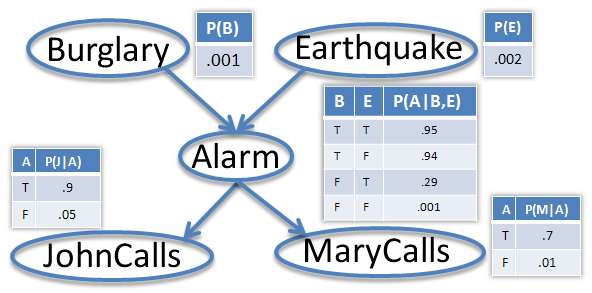
\includegraphics{alarm_bn_params.png} }% [clip=true, viewport= 1in 1in 9in 9in]
			\caption{First Bayes Net Example}
			\label{bnexample}
		\end{center} 
	\end{figure*} 
}



\problem{35}{
	The second part of the homework consists of implementing the key parts of the message passing algorithm in a more scalable object oriented setting.  The graph is set up for the large ALARM network in Figure~\ref{ALARM} .   The ALARM network is a network for monitoring patients in intensive care \footnote{http://compbio.cs.huji.ac.il/Repository/Datasets/alarm/alarm.htm}.  The graph is set up for you in the m-file object\_oriented\_algorithm/main\_big\_alarm\_net.m.  This code base makes extensive use of objects.  An object called node is defined in the folder @node and two specific nodes are then refined, namely @factor\_node and @variable\_node.  The refined objects inherit properties and methods from the general @node object unless they are specifically overwritten.  You will need to familiarize yourself will all three objects to be able to do the project.  There is also one other object called factor for this project.  A factor object is an object to hold the factor matrix, basically the probability tables.  Finally, you are provided a utility function called multilinear\_product.m which you may find useful.  You should read the comments at the top of the function which describe its functionality.  The last thing you need to know is that if $f$ is the factor matrix inside the factor object fn\_a\_b\_c then $f(1,3,2)$ is the factor value of f(a = 1, b = 3, c = 2).  Inside each factor node object, the list of neighboring objects is listed in exactly the same way for all factor nodes.  That is,  for fn\_a\_b\_c the neighboring nodes list will be $\{$vn\_a, vn\_b, vn\_c$\}$.\\
	
	The first task in this section of the HW will be to understand the code.  Then, you will need to implement the method {\bf getMessage(obj, to\_unid)} in both the factor\_node and variable\_node objects.  This will take some creativity and may require you to use a recursive function of make use of the eval function in MATLAB. You also need to implement the method {\bf getMarginalDistribution(obj)} in the variable\_node class definition. Finally, set up the main file to calculate the probability of KinkedTube given SaO2 is set to 1, BP is set to 1, ArtCO2 is set to 1, Press is set to 2, and ExpCO2 is set to 1.
	
	Because the network is actually loopy, we have to perform loopy inference here, but it is not critical that you understand how this is implemented.  At the bottom of the file object\_oriented\_algorithm/main\_big\_alarm\_net.m you can see an example of inference in the model after setting some specific values.\\
	
	\begin{figure*}
		\begin{center}
			\scalebox{.6}{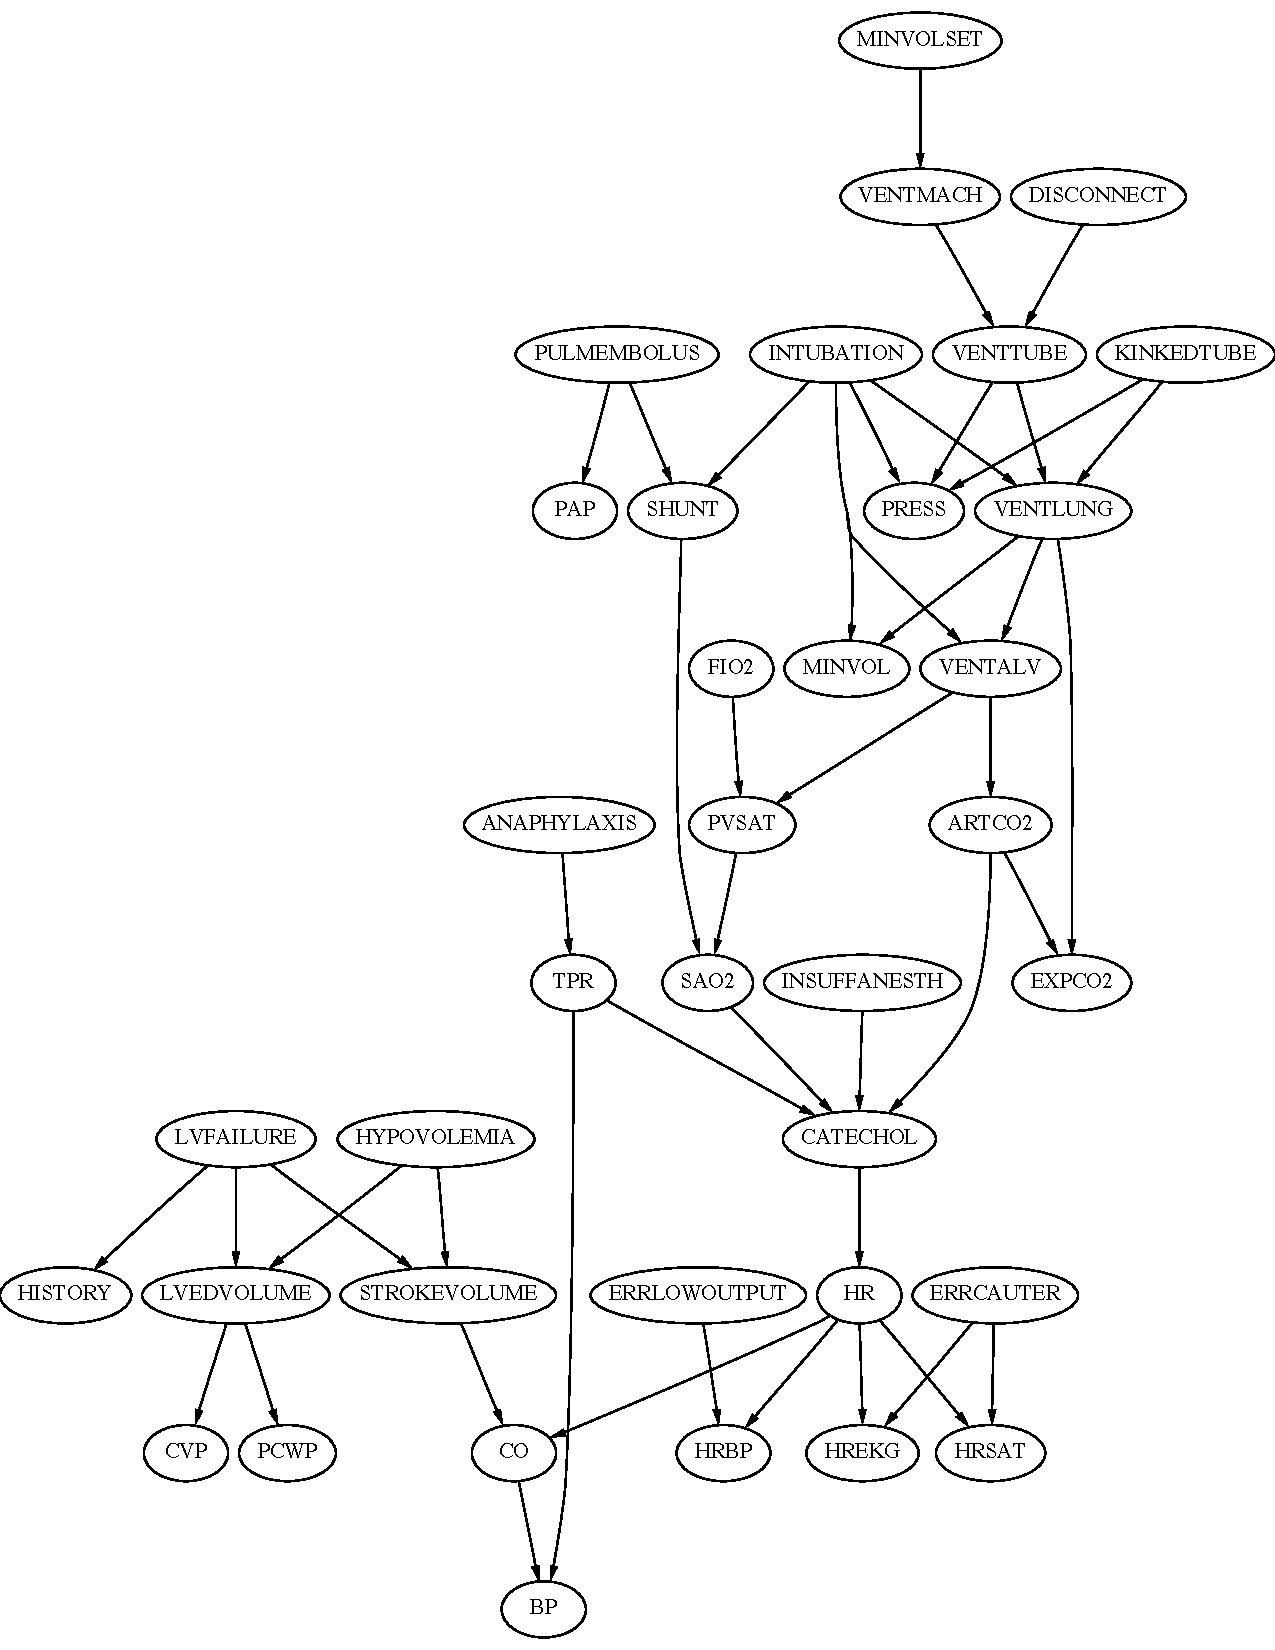
\includegraphics{alarm.pdf} }
			\caption{ALARM Bayes Net Example}
			\label{ALARM}
		\end{center} 
	\end{figure*} 
} 

{\bf Submitting your HW}

You must complete this HW assignment on your own, you are not permitted to work with any one else on the completion of this task.  Your grade will reflect your ability to implement a working version of the procedure.  Submitted code must run on my machine in less than 3 minutes.  Grading will be automated and the submitted files will be run, therefore to submit the HW you will need to follow the following directions exactly.

\begin{enumerate}
	\item Send an email to w4240.fall2010.stat.columbia.edu@gmail.com
	\item {Attach your updated MATLAB files 
		\begin{enumerate}
			\item explicit\_algorithm/main\_alarm\_network.m
			\item explicit\_algorithm/get\_marginal\_distribution.m
			\item explicit\_algorithm/get\_message\_fn\_aj.m 
			\item explicit\_algorithm/get\_message\_fn\_am.m 
			\item explicit\_algorithm/get\_message\_fn\_b.m 
			\item explicit\_algorithm/get\_message\_fn\_bea.m
			\item explicit\_algorithm/get\_message\_fn\_e.m
			\item explicit\_algorithm/get\_message\_vn.m
			\item object\_oriented\_algorithm/main\_big\_alarm\_net.m
			\item object\_oriented\_algorithm/@factor\_node/factor\_node.m
			\item object\_oriented\_algorithm/@variable\_node/variable\_node.m
		\end{enumerate} It is imperative that the names be exactly as described here. There should be no folders attached, only raw .m files.  You may not attach other MATLAB code files. }
	\item The subject will be exactly your Columbia UNI followed by a colon followed by hw2.  For example, if the TA were submitting this homework the subject would read {\bf nsb2130:hw2}
	\item If you submit hw more than once, later files will overwrite earlier files.
\end{enumerate}

% Problems End Here % ------------------------------------------------------- %

\problemsdone
\end{document}

% End of the Document
